\subsection{Pix2Pix-Kernkonzepte}
\subsubsection{Architektur des Generators}
Die Bildverarbeitung hat in den letzten Jahren durch den Einsatz tiefer neuronaler Netzwerke erhebliche Fortschritte gemacht. Im Mittelpunkt vieler dieser Fortschritte steht die U-Net-Architektur, die speziell für die Bildsegmentierung entwickelt wurde. Diese Architektur zeichnet sich durch ihre ausgeklügelte Kombination aus Encoder- und Decoder- Strukturen sowie durch den Einsatz von Skip-Verbindungen aus \cite{PhillipIsola.}. 
 \newline
Bei der Encoder-Decoder-Struktur handelt es sich um einen Ansatz, bei dem das Eingangsbild zunächst durch den Encoder schrittweise reduziert wird. Dieser Prozess dient dazu, wesentliche Merkmale des Bildes zu erfassen. Anschließend wird das Bild durch den Decoder wiederhergestellt, indem die zuvor extrahierten Merkmale verwendet werden. Während dieser Prozesse besteht jedoch das Risiko des Informationsverlustes, insbesondere in den tieferen Schichten des Netzwerks.
Um dieses Problem zu adressieren, führt die U-Net-Architektur Skip-Verbindungen ein. Diese direkten Verbindungen zwischen korrespondierenden Schichten des Encoders und Decoders sorgen dafür, dass Detailinformationen nicht verloren gehen. Genauer gesagt, ermöglichen diese Verbindungen den direkten Informationsfluss zwischen jeweils äquivalenten Schichten, wodurch die Rekonstruktion des Bildes im Decoder mit einer höheren Genauigkeit erfolgt\cite{PhillipIsola.}. \newline
Die Bedeutung von Skip-Verbindungen zeigt sich insbesondere in Anwendungen wie der Bild-zu-Bild-Übersetzung. Hier muss oft ein Bild mit niedriger Auflösung in ein Bild mit hoher Auflösung überführt werden, ohne dass Details verloren gehen. Die U-Net-Architektur, die angereichert mit diesen Verbindungen ist, ermöglicht daher eine feinere Rekonstruktion, die sowohl globale als auch lokale Informationen berücksichtigt \cite{PhillipIsola.}.  \newline
Somit kann die U-Net-Architektur durch ihre Kombination aus Encoder-Decoder-Struktur und Skip-Verbindungen ein effektives Werkzeug für die Bildsegemtierung darstellen. Ihre Fähigkeit, sowohl globale Muster als auch feine Details zu berücksichtigen, macht sie zu einer bevorzugten Wahl für viele Bildverarbeitungsaufgaben \cite{PhillipIsola.}. \newline
In Abbildung \ref{fig:unet} ist die typische U-Net-Architektur dargestellt. Die linke Seite des ''U'' repräsentiert den Encoder-Teil, der das Eingangsbild schrittweise reduziert und wesentliche Merkmale extrahiert. Die rechte Seite repräsentiert den Decoder-Teil, der das Bild mithilfe der extrahierten Merkmale rekonstruiert. Die horizontalen Linien repräsentieren die Skip-Verbindungen, die sicherstellen, dass Detailinformationen zwischen den korrespondierenden Schichten des Encoder und Decoders direkt übertragen werden \cite{PhillipIsola.}. \newline 
In der Pix2Pix Technologie fungiert die U-Net-Architektur als zentraler Bestandteil des Generators, verantwortlich für die Bild-zu-Bild-Übersetzung. Die Wahl von U-Net für diesen Zweck basiert auf seiner Fähigkeit, feinere Details und Kontextinformationen aus dem Eingangsbild zu bewahren, was für die Qualität der Bild-zu-Bild-Übersetzung ausschlaggebend ist. Der Generator nutzt die Encoder-Decoder-Struktur von U-Net, um den globalen Kontext des Bildes zu erfassen, während die Skip-Verbindungen sicherstellen, dass auch lokale Details im resultierenden Bild erhalten bleiben. Diese Eigenschaften machen U-Net zu einem effektiven Werkzeug innerhalb des Generators, indem sie eine hohe Detailtreue und Kontextsensitivität in der Bild-zu-Bild-Übersetzung ermöglichen\cite{PhillipIsola.}.

\begin{figure}[h]
	\centering
	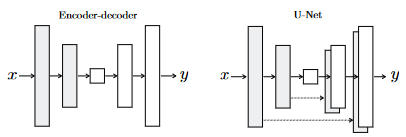
\includegraphics[width=0.7\linewidth]{./images/unet.png}
	\caption{Schematische Darstellung der U-Net-Architektur. Die Architektur besteht aus einem Encoder-Teil (links), einem Decoder-Teil (rechts) und Skip-Verbindungen zwischen korrespondierenden Schichten.}
	\label{fig:unet}
\end{figure}

\subsubsection{Architektur des Diskriminator}
\label{sec:PatchGAN}
Im Kontext von Pix2Pix GANs, spielt der PatchGAN-Diskriminator eine besonders wichtige Rolle. Der zentrale Unterschied dieses Diskriminators zu allgemeinen Diskriminatoren liegt in der Art und Weise, wie er Bilder bewertet. Statt das gesamte Bild zu beurteilen, zerlegt der PatchGAN-Diskriminator das Bild in mehrere kleinere Bildabschnitte oder Patches und bewertet jeden Patch einzeln auf seine Echtheit \cite{PhillipIsola.}. \newline
Ein solches Vorgehen hat den klaren Vorteil, dass feinere Strukturen und Details in den Bildern erkannt und beurteilt werden können. Durch diese segmentierte Beurteilung kann der Diskriminator besser einschätzen, ob die Struktur und Beschaffenheit eines bestimmten Bildteils realistisch ist. Dies ist besonders nützlich, da kleinere Unstimmigkeiten in den Bildern, die ein allgemeiner Diskriminator möglicherweise übersieht, vom PatchGAN erfasst werden können. \newline
Ein weiterer Vorteil des PatchGAN-Diskriminators ist seine Skalierbarkeit. Da er auf festen Patchgrößen basiert, kann er flexibel auf Bilder unterschiedlicher Größen angewendet werden, ohne dass das zugrunde liegende Modell geändert werden muss. Dies führt nicht nur zu einer schnelleren Bildverarbeitung, sondern ermöglicht auch eine effiziente Ausführung auf großen Bildern. Darüber hinaus reduziert es potenzielle Kachelartefakte, die bei allgemeinen Diskriminatoren auftreten können \cite{PhillipIsola.}.\newline
Der PatchGAN-Diskriminator kann wenn er effektiv eingesetzt wird, zu besseren und realistischeren Bildern im adverseriellen Lernprozess beitragen. Seine Fähigkeit, lokale Bildinformationen zu bewerten, ermöglicht es auch subtile Unterschiede in den Bildern zu erkennen, was zu einer verbesserten Qualität der generierten Bilder führt \cite{PhillipIsola.}.
\footnote[1]{https://towardsdatascience.com/cyclegan-learning-to-translate-images-without-paired-training-data-5b4e93862c8d}

\begin{figure}[h]
	\centering
	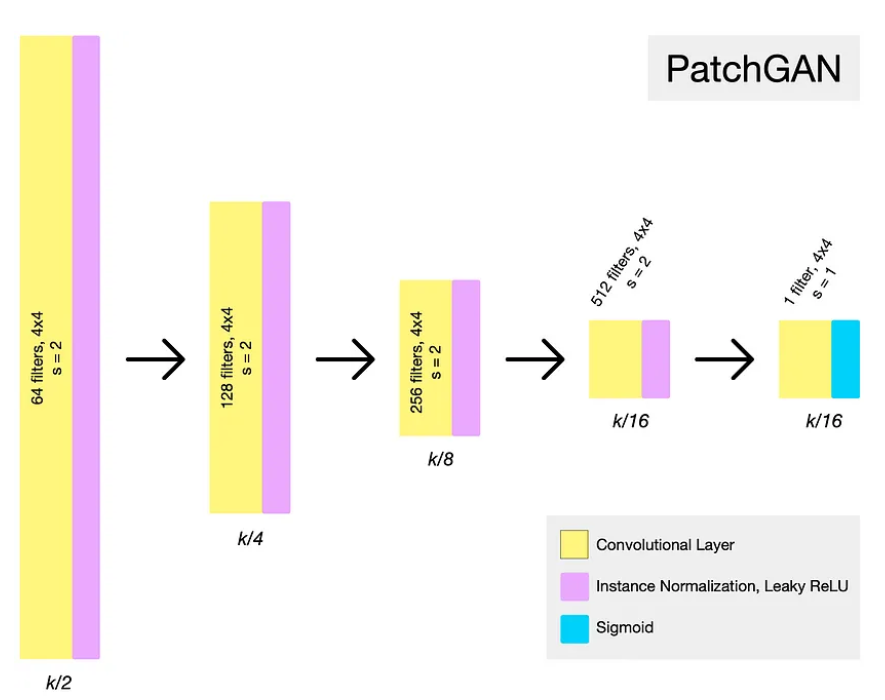
\includegraphics[width=0.7\linewidth]{./images/cycleGanDiscriminatorArchitecutre.png}
	\caption{Eine mögliche Architektur eines PatchGAN Diskriminator\protect\footnotemark[1]}
	\label{fig:PatchGANDiskriminator}
\end{figure}
\newpage

\subsubsection{L1-Verlustfunktion}

Die L1-Verlustfunktion, auch bekannt als Mean Absolute Error (MAE), spielt eine entscheidende Rolle im Pix2Pix-Modell, einem bedingten Generative Adversarial Network (cGAN) für Bild-zu-Bild-Übersetzungen. Diese Verlustfunktion misst den durchschnittlichen absoluten Unterschied zwischen den vorhergesagten und den tatsächlichen Werten, wodurch sie die Genauigkeit der generierten Bilder verbessert, insbesondere im Hinblick auf die niedrigen Frequenzen im Bild. Die L1-Verlustfunktion trägt somit maßgeblich zur Bewahrung der strukturellen Integrität und des Kontexts des Bildes bei \cite{PhillipIsola.}. \newline
Die Verwendung des L1-Verlusts zusätzlich zum adversariellen Verlust im Pix2Pix-Modell ist von entscheidender Bedeutung. Während der adversarielle Verlust darauf abzielt, die generierten Bilder realistisch erscheinen zu lassen, konzentriert sich der L1-Verlust auf die Genauigkeit der niedrigen Frequenzen, um die strukturelle Integrität und den Kontext des Bildes zu bewahren. Diese Kombination aus der l1-Verlustfunktion und dem adversariellen Verlust im Pix2Pix-Modell ermöglicht es, sowohl die niedrigen als auch die hohen Frequenzen im Bild effektiv zu erfassen, was zu generierten Bildern führt, die sowohl strukturell korrekt als auch visuell ansprechend sind \cite{PhillipIsola.}. \newline
Die L1-Verlustfunktion neigt jedoch dazu, bei den hohen Frequenzen unscharfe Ergebnisse zu liefern. Dies liegt daran, dass der L1-Verlust den Median der möglichen Werte bevorzugt, was zu einer Glättung der Bildtexturen führen kann. Um dieses Problem zu adressieren und scharfe, hochfrequente Details im Bild zu erhalten, wird der L1-Verlust im Pix2Pix-Modell mit einem adversariellen Verlust kombiniert. Diese synergetische Kombination von Verlustfunktionen ermöglicht es dem Pix2Pix-Modell, hochwertige Bild-zu-Bild-Übersetzungen durchzuführen, die sowohl visuell ansprechend als auch strukturell korrekt sind \cite{PhillipIsola.}. \newline
Darüber hinaus hat sich die Kombination von L1-Verlust und adversariellen Verlust im Pix2Pix-Modell als nützlich für eine Vielzahl von Bild-zu-Bild-Übersetzungs-problemen erwiesen, einschließlich semantischer Segmentierung und Farbgebung. Durch die effektive Erfassung sowohl der niedrigen als auch der hohen Frequenzen im Bild trägt das Pix2Pix-Modell dazu bei, die Qualität der generierten Bilder zu verbessern und ihre Anwendbarkeit auf verschiedene Probleme zu erweitern \cite{PhillipIsola.}.

\subsubsection{Training}

Der Trainingsprozess von Pix2Pix-Generative Adversarial Networks in der Bild-zu-Bild-Übersetzung geht über die bloße Erlernung der Abbildung von Eingabe- zu Ausgabebildern hinaus. Er umfasst auch das Entwickeln einer Verlustfunktion, die speziell auf diese Art der Bildtransformation abgestimmt ist. Pix2Pix benötigt eine spezifische Art von Trainingsdaten, um effektiv zu funktionieren. Die Trainingsdaten bestehen aus Paaren von Bildern, wobei jedes Paar ein Eingabebild und das entsprechende Ausgabebild enthält. Diese Bilder können eins bis drei Kanäle aufweisen, was bedeutet, dass das Modell sowohl mit monochromatischen (Graustufen) als auch mit farbigen Bildern (RGB) arbeiten kann.
Im Rahmen des Trainingsprozesses von Pix2Pix wird eine iterative Methode verwendet, bei der der Generator und der Diskriminator abwechselnd traininert werden.
Eine Schlüsselkomponente dieses Prozesses ist die Verwendung einer zusammengesetzten Verlustfunktion, die sowohl den adverseriellen Verlust (bewertet vom Diskriminator) als auch den L1-Verlust(mittlerer absoluter Fehler zwischen generiertem Bild und Zielbild) umfasst. Dadurch wird der Generator dazu angehalten, realistische Übersetzungen der Eingabebilder zu generieren. Dieses Gleichgewicht zwischen Generator und Diskriminator ist entscheidend für die Effektivität des Pix2Pix-Modells \cite{HazemAbdelmotaalAhmedA.AbdouAhmedF.OmarDaliaMohamedElSebaityKhaledAbdelazeem.2021}.\newline
Im Pix2Pix-Modell spielt die Batch-Normalisierung eine wesentliche Rolle für die Stabilisierung des lernprozesses. Anstatt herkömmliche Batch-Normalisierungstechniken zu verwenden, setzt Pix2Pix auf $Instance\ Normalization$, bei der die Statistiken jedes Testbatches statt der aggregierten Trainingsbatch-Statistiken genutzt werden. Diese Methode hilft, Variation in den Aktivierungen zwischen verschiedenen Bildern zu reduzieren, was für die Bildgenerierungsaufgabe von Vorteil ist. \newline
Diese Normalisierung ergänzt die iterative Trainingsmethode von Pix2Pix, bei der Generator und Diskriminator abwechselnd trainiert werden. Sie ist besonders wichtig, da der Generator mit einer Vielzahl von Eingabedaten, einschließlich monochromatischer und farbiger Bilder, arbeitet. Zusammen mit der zusammengesetzten Verlustfunktion, die aus adverseriellem und L1-Verlust besteht, verbessert die Batch-Normalisierung die Trainingsstabilität und Qualität der generierten Bilder \cite{PhillipIsola.}. 
  

